\documentclass{beamer}
\beamertemplatenavigationsymbolsempty
\usecolortheme{beaver}
\setbeamertemplate{blocks}[rounded=true, shadow=true]
\setbeamertemplate{footline}[page number]
%
\usepackage[utf8]{inputenc}
\usepackage[english,russian]{babel}
\usepackage{amssymb,amsfonts,amsmath,mathtext}
\usepackage{subfig}
\usepackage[all]{xy} % xy package for diagrams
\usepackage{array}
\usepackage{multicol} % many columns in slide
\usepackage{hyperref} % urls
\usepackage{hhline} %tables
\usepackage{comment} %comments
% Your figures are here:
\graphicspath{ {fig/} {../fig/} }

%----------------------------------------------------------------------------------------------------------

\title[\hbox to 56mm{Классификация траекторий физических систем}]{Классификация траекторий физических систем\\ с помощью лагранжевых нейронных сетей}
\author[А.\,И.~Богданов]{Александр Иванович Богданов}
\institute{Московский физико-технический институт}
\date{\footnotesize
\par\smallskip\emph{Курс:} Моя первая научная статья
\par\smallskip\emph{Эксперт:} В.\,В.~Стрижов
\par\smallskip\emph{Консультант:} С.\,К.~Панченко
\par\bigskip\small 2023}

%----------------------------------------------------------------------------------------------------------

\begin{document}

%----------------------------------------------------------------------------------------------------------

\begin{frame}

    \thispagestyle{empty}
    \maketitle
    
\end{frame}

%-----------------------------------------------------------------------------------------------------

\begin{frame}{Цель исследования}
    \begin{block}{Цель}
        Исследование методов решения задачи классификации.
    \end{block}
    \begin{block}{Задача}
        Решение задачи классификации с помощью лагранжевой нейронной сети.
    \end{block}
    \begin{block}{Решение}
        Моделирование обобщенного лагранжиана и последующим сравнением полученных коэффициентов для определения вида активности на датасете PAMAP2.
    \end{block}
\end{frame}

%-----------------------------------------------------------------------------------------------------

\begin{frame}{Публикации по теме}
    \begin{itemize}
    
    \item Северилов Павел. Выбор оптимальной модели в задаче моделирования динамики физической системы. \url{https://github.com/severilov/master-thesis}.

    \item Miles Cranmer, Sam Greydanus, Stephan Hoyer, Peter Battaglia, David Spergel, and Shirley Ho. Lagrangian neural networks. arXiv preprint arXiv:2003.04630, 2020.
  
    \end{itemize}
\end{frame}

%-----------------------------------------------------------------------------------------------------

\begin{frame}{Задача регрессии динамики физической системы}

    Задана выборка из точек траектории $\{\mathbf{x}_i, \mathbf{y}_i\}$, где $\mathbf{x}_i = (\mathbf{q}_i, \mathbf{\dot{q}}_i)$,  $\mathbf{{y}}_i = \mathbf{\dot{x}}_i = (\mathbf{\dot{q}}_i, \mathbf{\ddot{q}}_i)$
    
    Регрессионная модель выбирается из класса нейронных сетей:
    $$\mathbf{f} \colon (\mathbf{w}, \mathbf{X}) \to \hat{\mathbf{y}},$$ 
    
    Функцией ошибки взята квадратичная ошибка:
    $$\mathcal{L}(\mathbf{y}, \mathbf{X}, \mathbf{w}) = \| \hat{\mathbf{y}} - \mathbf{y} \|_2^2.$$

    Зафиксируем выборку $\mathcal{L}(\textbf{w}) = \mathcal{L}(\mathbf{y}, \mathbf{X}, \mathbf{w})$.
    
    Задача моделирования динамики системы представлена в виде задачи минимизации квадратичной ошибки: 
    $$\textbf{w}^* = \arg \min_{\mathbf{w}\in\mathbb{W} }\left(\mathcal{L}(\textbf{w})\right).$$


\end{frame}

%----------------------------------------------------------------------------------------------------------

\begin{frame}{Задача классификации физических траекторий}

    Выборка $H = \{\text{L}_i(\textbf{w}^*)\}_{i = 1}^n$ - множество объектов с известными метками, где каждый объект - обобщенный лагранжиан.
    
    С помощью известных классификаторов решается задача: $\textbf{L}(\textbf{w}^*) \rightarrow \{1 \dots K\}$.


\end{frame}

%----------------------------------------------------------------------------------------------------------

\begin{frame}{Подготовка данных}

    Для эксперимента используется датасет PAMAP2. В нём есть несколько проблем:
        \begin{itemize}
    
            \item Пропуски данных, связанные с тем, что датчик может пропустить такт. Для восстановления данных использовалась сплайн-интерполяция.

            \item Отсутствие необходимых данных: ускорения и координаты. Для их получения использовались методы вычислительной математики.

            Для получения ускорения:
            $$f'(x_i) \approx \frac{f(x_{i + 1}) - f(x_{i - 1})}{2h}$$.

            Для получения координаты:
            $$\int\limits_a^b f(x) dx \approx \frac{h}{3} \sum\limits_{k = 1}^{N - 1} \left( f(x_{k + 1} + 4f(x_k) + f(x_{k - 1}) \right)$$

        \end{itemize}

\end{frame}

%----------------------------------------------------------------------------------------------------------

\begin{frame}{Вычислительный эксперимент}

    Датасет:
        \begin{itemize}

            \item Акселерометры:
                    \begin{itemize}

                        \item На запястье рабочей руки

                        \item На рабочей ноге

                        \item На груди

                    \end{itemize}

            \item Частота акселерометров: 100 Гц.
            
            \item Количество классов: K = 24, используется 4.

        \end{itemize}
        
Фиксируется подвыборка из датасета PAMAP2. Для каждого объекта строится обобщенный лагранжиан. С помощью различных классификаторов определяем принадлежность к какому-либо классу.
Понижается размерность данных, а затем строится график распределения данных.

\end{frame}

%----------------------------------------------------------------------------------------------------------

\begin{frame}{Анализ ошибки}

    Распределение классов:

        \begin{columns}[c]
        
            \column{0.6\textwidth}
                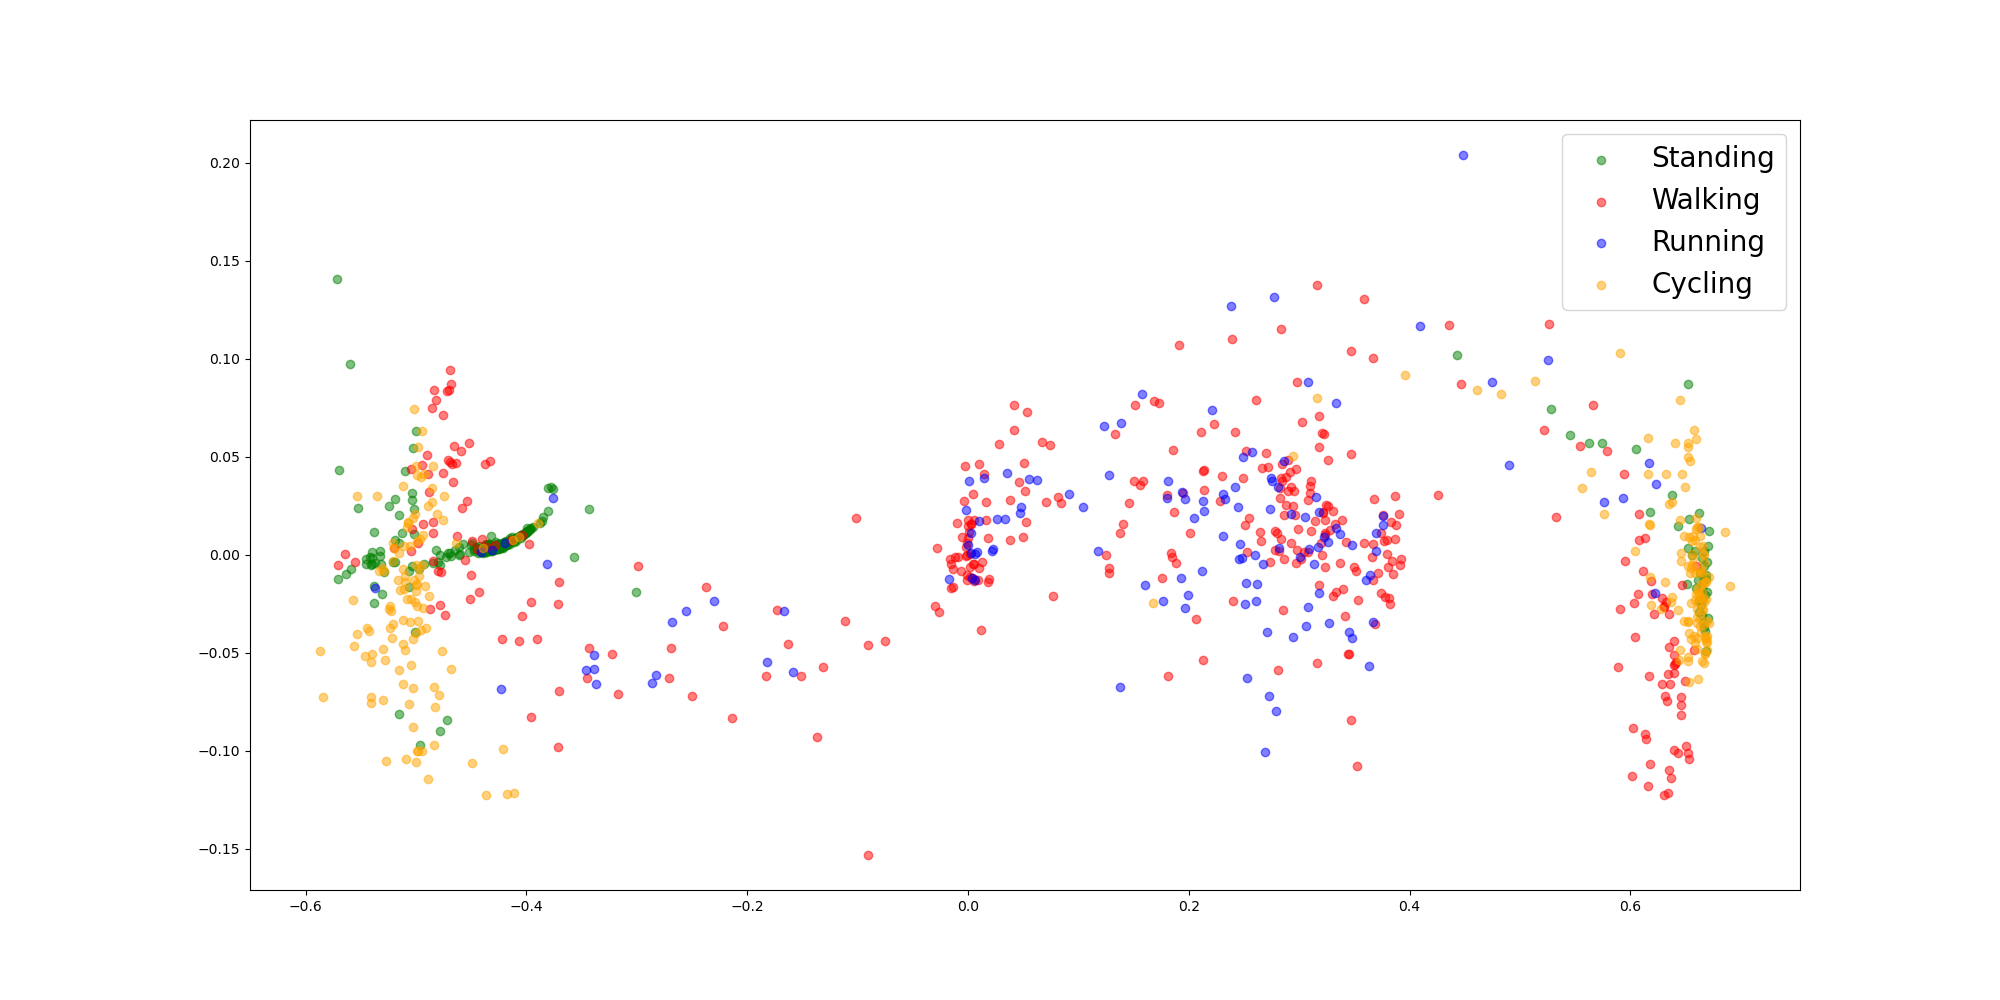
\includegraphics[width=1.1\textwidth]{Data}
                
            \column{0.6\textwidth}
                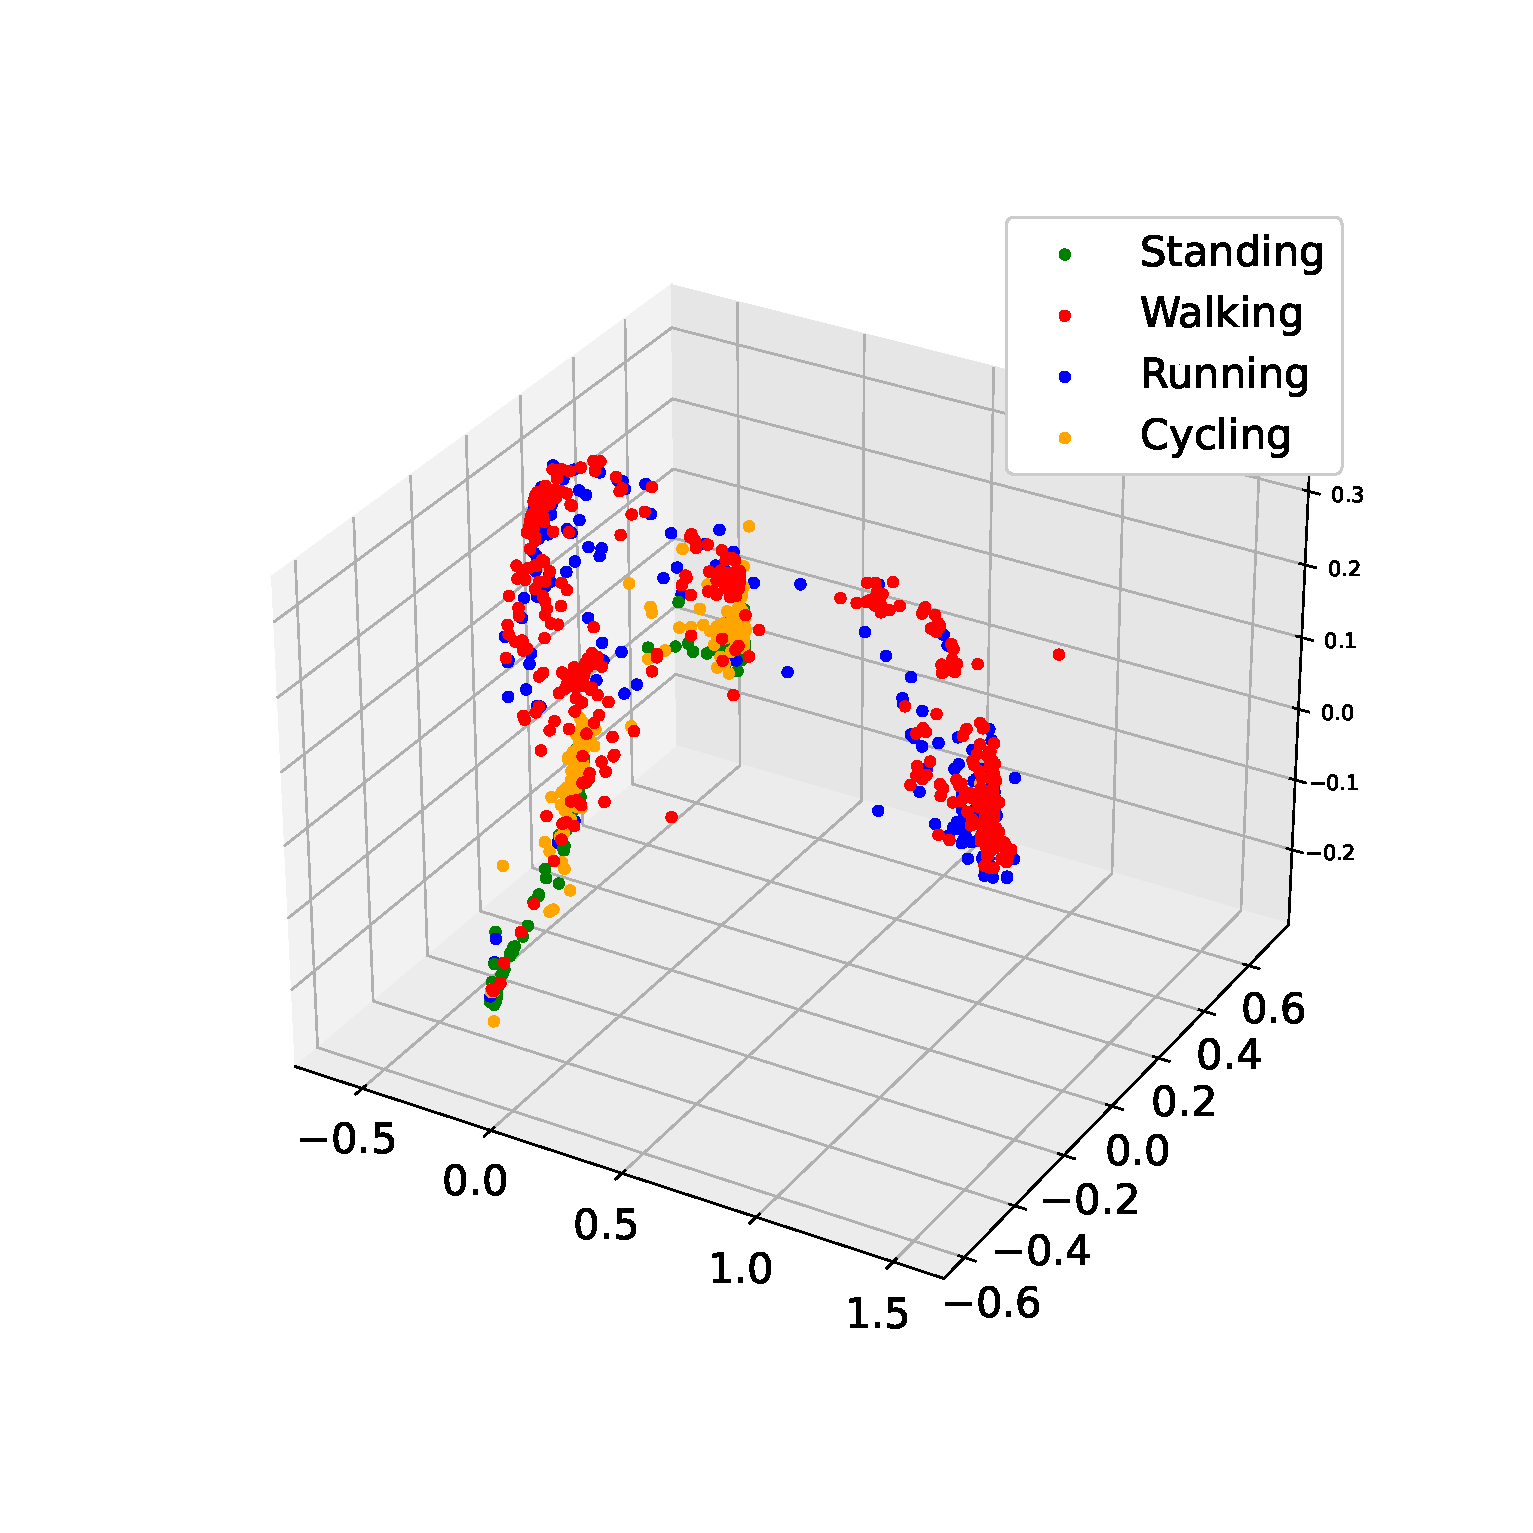
\includegraphics[width=1.3\textwidth]{Data_3D}
                
        \end{columns}

        Точность:

        \begin{columns}[c]
        
            \column{0.6\textwidth}
                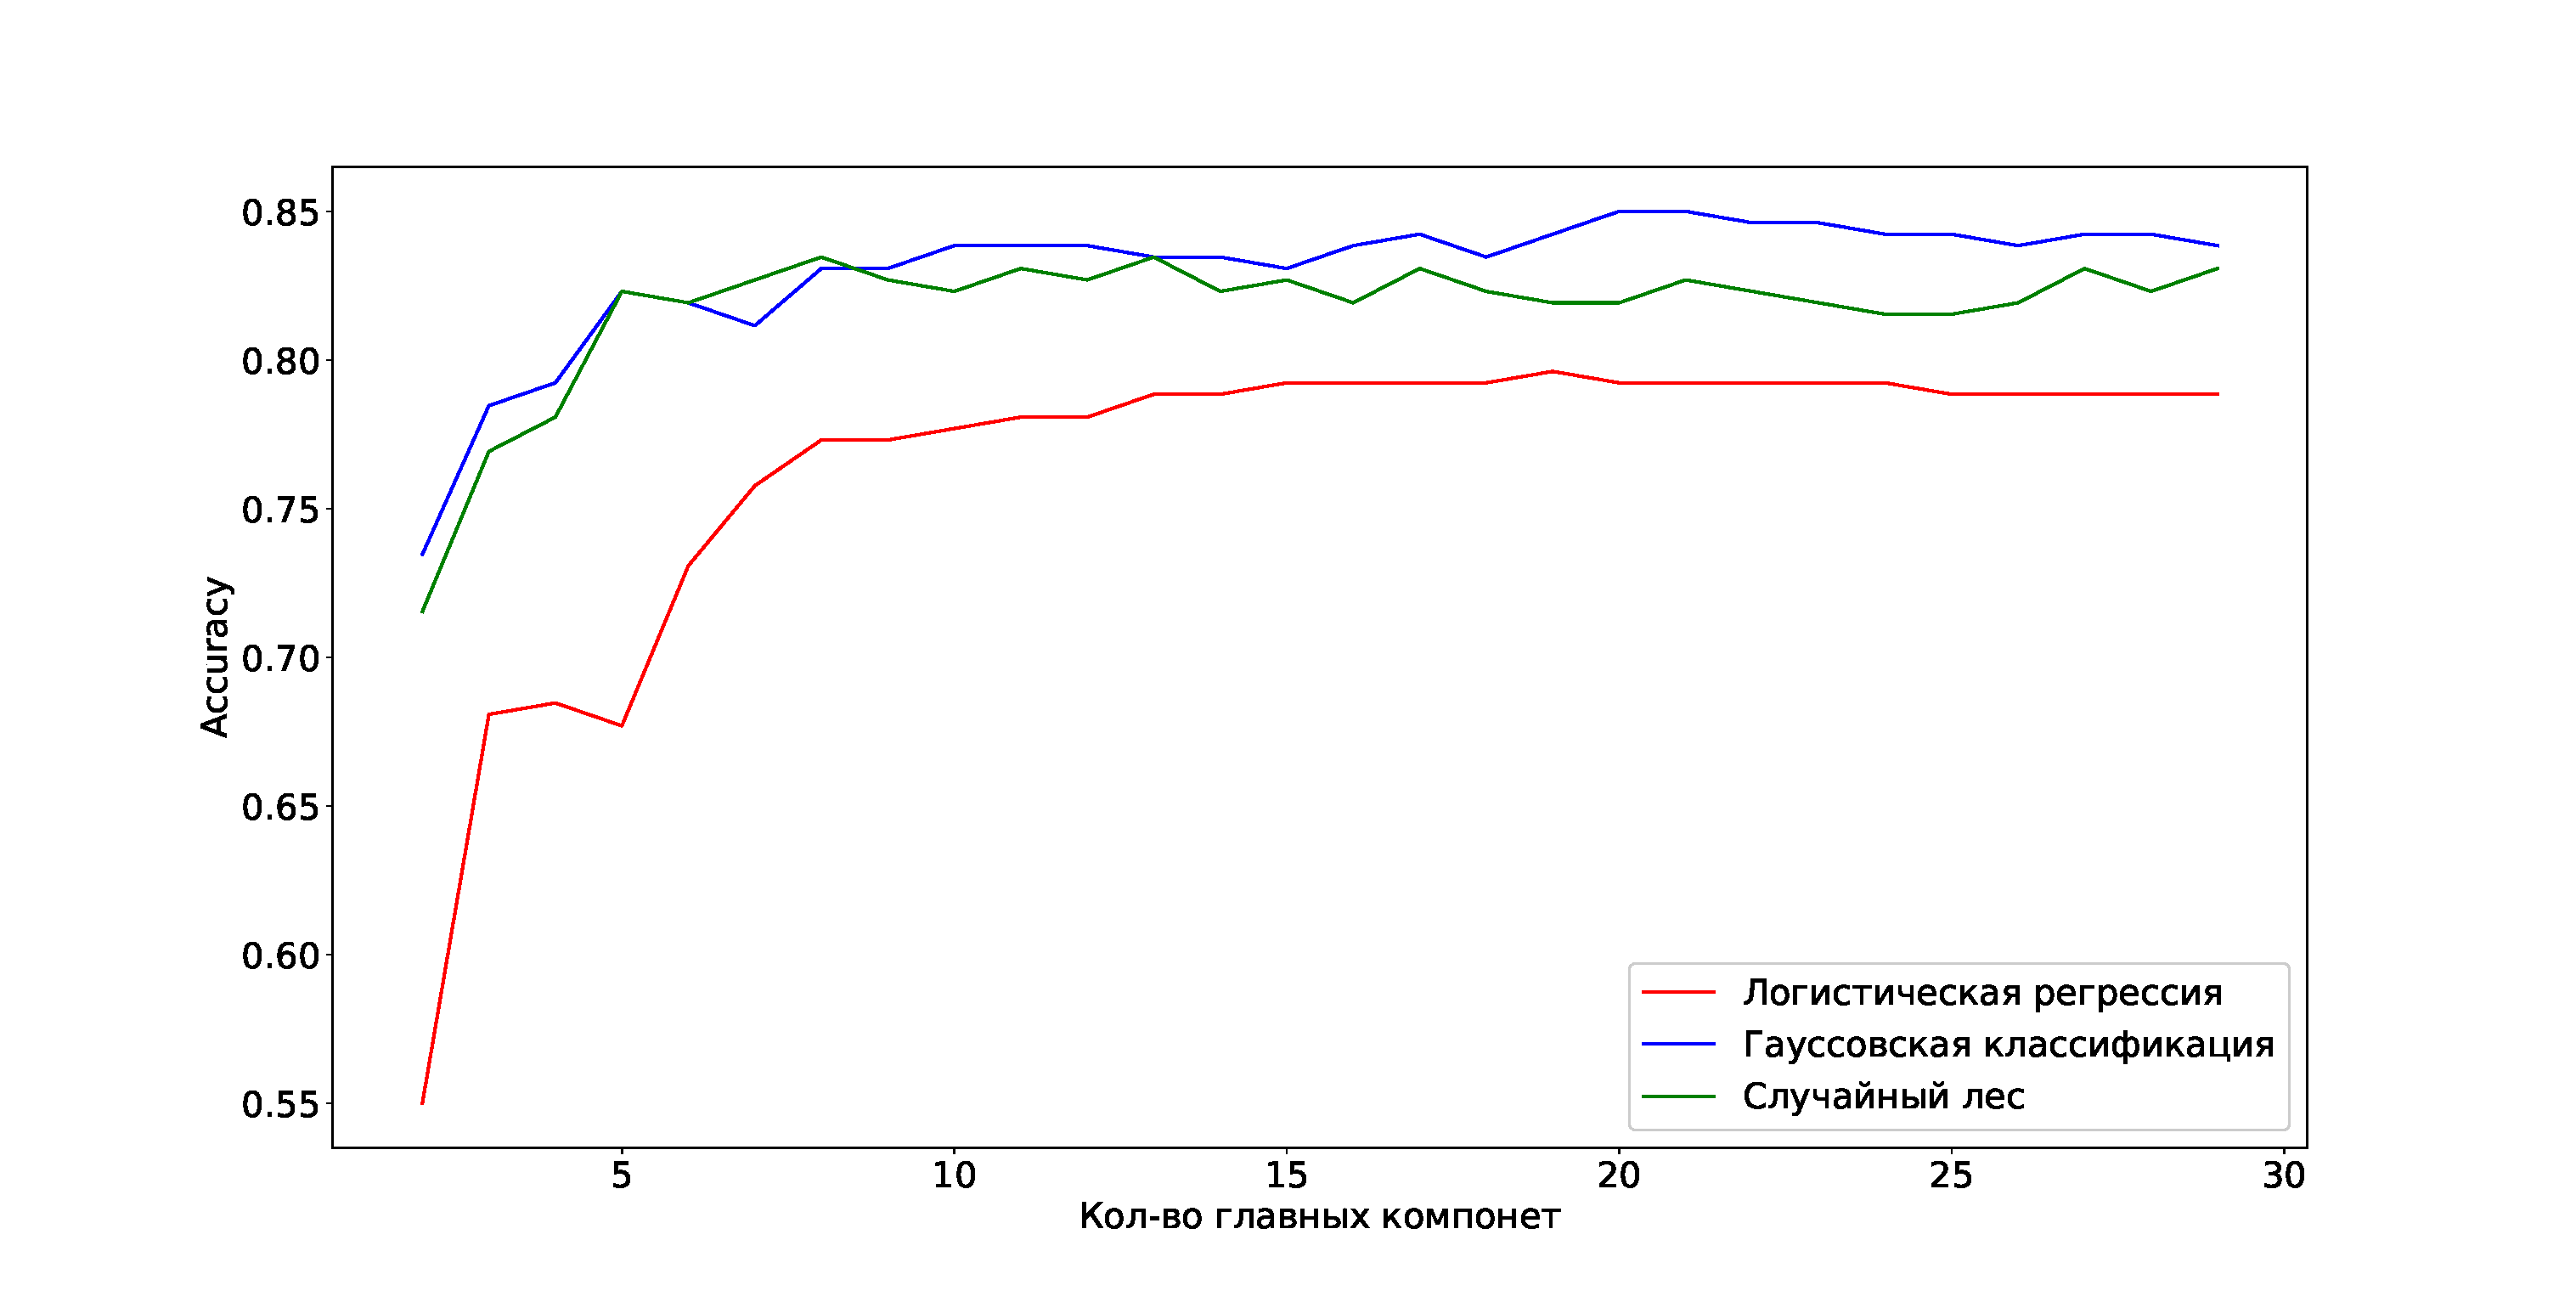
\includegraphics[width=1.0\textwidth]{Accuracy}
                
            \column{0.6\textwidth}
                    \begin{itemize}

                        \item LogisticRegression: 79$\%$

                        \item GaussianProcessClassifier: $86\%$

                        \item RandomForestClassifier: $85\%$

                    \end{itemize}
                
        \end{columns}


\end{frame}

%----------------------------------------------------------------------------------------------------------

\begin{frame}{Заключение}

    \begin{itemize}
    
        \item Предложен метод решения задачи классификации динамических систем с помощью лагранжевой нейронной сети.

        \item Проведен вычислительный эксперимент на датасате PAMAP2, который содержит данные о активности человека.
        
        \item Получено, что при использовании данного метода, получается хорошая точность предсказания.
        
    \end{itemize}
    
\end{frame}

%----------------------------------------------------------------------------------------------------------

\end{document} 